\section{La Qualité}

	%						%
	%  PREMIERE PARTIE		%
	%						%

\subsection{Présentation}

% Première slide %
\begin{frame}
  \frametitle{\color{white} Présentation}
  Liste des objets à test :
  \begin{itemize}
  \item L'interface graphique des fonctions GnuPG
  \item La visualisation de la toile de confiance
  \item L'implémentation de l'attaque sur les secondes pré-images
  \end{itemize}
\end{frame}

% Deuxième slide %
\begin{frame}
  \frametitle{\color{white} Environnement}
  \begin{itemize}
  \item Outils
  \item Jeux de données
  \item Contraintes
  \end{itemize}
  \begin{figure}[p]
    \centering
    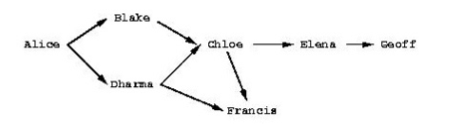
\includegraphics[scale=.40]{jeuxtest.png}
    \caption{Schéma données de test}
  \end{figure}
  
\end{frame}


	%						%
	%  SECONDE PARTIE		%
	%						%

\subsection{Les tests}
% Troisième slide %
\begin{frame}
  \frametitle{\color{white} Stratégies des tests}
  \begin{block}{Approche choisie pour les tests}
   Ecriture des tests automatisés puis écriture du code pour faire passer le test
  \end{block}
  \begin{figure}[p]
    \centering
    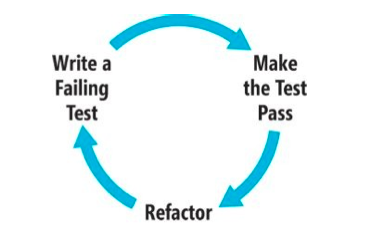
\includegraphics[scale=.25]{tests.png}
    \caption{Développement dirigé par les tests}
  \end{figure}
\end{frame}

% Quatrième slide %
\begin{frame}
  \frametitle{\color{white} Gestion des anomalies}
  \begin{block}{Principales étapes lors d'une anomalie}
  \begin{itemize}
  \item Création d'un mémo
  \item Ajout d'une entrée au journal
  \item Diffusion de la note
  \item Désignation de la personne pour corriger
  \item Correction de l'erreur
  \item Vérification et création d'un contre-mémo
  \end{itemize}
  \end{block}
\end{frame}


